%!TEX TS-program = pdflatex
\documentclass{beamer}
\usepackage{beamerthemeshadow}
\usepackage[T1]{fontenc} 
\usepackage{fixltx2e}
\usepackage[brazil]{babel}
\usepackage{lmodern}
\usepackage[utf8]{inputenc}
\usepackage[english]{babel}
\usepackage{amsmath,amssymb,amsfonts,amsthm}
\usepackage[makeroom]{cancel}
\usepackage{graphicx}
\usepackage{wrapfig}
\usepackage{hyperref}
\usepackage{color}
\usepackage{colortbl}
\usepackage{xmpmulti}
\usepackage{multirow}
\usepackage{mdwtab}
\usepackage{verbatim}

%PACKAGE ADDED IN ORDER TO SHOW EXIT LOCATION SYMBOLS
\usepackage{pifont}
\usepackage{marvosym}
%IMPROVES WHITESPACING AROUND "..."
\usepackage{ellipsis}         
%ADDS THE 'SMILE FACE'
\usepackage{wasysym} 
%ADDS STRIKETHROUGH FONT
\usepackage{ulem}
\DeclareRobustCommand{\hsout}[1]{\texorpdfstring{\sout{#1}}{#1}}

\pdfpkresolution=2400

%USEFUL FOR HIGHLIGHTING TEXT AND CODE
\usepackage{tikz}
\usetikzlibrary{positioning,calc,arrows,shapes,shadows,trees}
\tikzset{onslide/.code args={<#1>#2}{%
  \only<#1>{\pgfkeysalso{#2}} % \pgfkeysalso doesn't change the path
}}
\usepackage{smartdiagram}

\usepackage{microtype}


\title{Uma abordagem para criação, reúso e aplicação de refatorações no contexto da modernização dirigida a arquitetura}

\date{}

\author{Rafael Serapilha Durelli\\Orientador: Prof. Dr. Márcio Eduardo Delamaro}


\institute{USP - ICMC\\
\Letter\{rdurelli, delamaro\}@icmc.usp.br
}
\titlegraphic{
\includegraphics[width=0.4\textwidth]{figures/figuraLocais.pdf}} %,height=0.12\textheight
\makeindex

\newcommand{\nl}{\ \par \noindent }
\newcommand{\hl}[1]{\textbf{#1}}
\newcommand{\hll}[1]{\underline{#1}}

\usetheme{Warsaw}
% \titlegraphic{\scalebox{0.125}{\includegraphics{fapesp_logo.pdf}}}

%PRESENTATION
\begin{document} 

%SHOW SLIDE NUMBER
\setbeamertemplate{footline}[frame number]

%PRESENTATION TITLE
\frame[label=firstslide]{\maketitle}


\begin{frame}{Agenda}
\tableofcontents
\end{frame}


\section{Introdução}
\label{sec:introducao}

\subsection{Contextualização, Motivações, Objetivos e Sínteses da Pesquisa Conduzida}

%\subsection{Objetivos e Sínteses da Pesquisa Conduzida}

\begin{frame}\frametitle{Introdução - Contextualização}

\begin{block}{Sistemas Legados (SL)}
\begin{minipage}[b]{10.80cm}
São aqueles cujos custos de manutenção e evolução encontram-se fora dos níveis aceitáveis para uma organização, mas que ainda são úteis para apoiar seus processos internos.
\end{minipage}  
\end{block}

\begin{itemize}
    \begin{minipage}[b]{9.8cm} \item Sistemas Legados; 
    \vspace{.2cm}
        \begin{itemize}
            \begin{minipage}[b]{9.8cm} \item Documentação inconsistentes; 
            \vspace{.2cm}
            \end{minipage}
            \begin{minipage}[b]{9.8cm} \item Dificulta sua manutenção; 
            \vspace{.2cm}
            \end{minipage}
            \begin{minipage}[b]{9.8cm} \item Substituí-lo é uma tarefa muito cara e propensa a erros. 
            \vspace{.2cm}
            \end{minipage}
        \end{itemize}
    \end{minipage}
    \begin{minipage}[b]{9.8cm} \item Uma alternativa à substituição de um SL são os tradicionais processos de reengenharia; 
    \vspace{.2cm}
        \begin{itemize}
            \begin{minipage}[b]{9.8cm} \item \textit{Object Management Group} (OMG) lançou em 2003 a ADM; 
            \vspace{.2cm}
            \end{minipage}
        \end{itemize}
    \end{minipage}
\end{itemize}

\end{frame}

\begin{frame}\frametitle{Introdução - Contextualização}

\begin{block}{\textit{Architecture-Driven Modernization} (ADM)}
\begin{minipage}[b]{10.80cm}
OMG definiu a ADM cujo objetivo principal é padronizar processos de reengenharia por meio de metamodelos padronizados~\cite{KDM:specification,KDM:ISO}.
\end{minipage}  
\end{block}

\begin{block}{\textit{Knowledge Discovery Metamodel} (KDM)}
\begin{minipage}[b]{10.80cm}
Knowledge Discovery Metamodel (KDM) é o principal metamodelo da ADM. E possui uma ampla quantidade de metaclasses para representar diferentes níveis de abstração.
\end{minipage}  
\end{block}

\begin{itemize}
    \begin{minipage}[b]{9.8cm} \item Código-fonte; 
    \vspace{.2cm}
    \end{minipage}
    \begin{minipage}[b]{9.8cm} \item Arquitetura, regras de negócio e outros conceitos abstratos do sistema; 
    \vspace{.2cm}
    \end{minipage}
    \begin{minipage}[b]{9.8cm} \item GUI, arquivos de configuração, bases de dados, etc; 
    \vspace{.2cm}
    \end{minipage}
\end{itemize}

\end{frame}

\begin{frame}\frametitle{Introdução - Contextualização}

\begin{block}{\textit{Architecture-Driven Modernization} (ADM)}
\begin{minipage}[b]{10.80cm}
A ADM almeja que a comunidade comece a desenvolver algoritmos e técnicas que sejam dependentes e específicas apenas do metamodelo KDM, e não de plataformas, metamodelos proprietários ou linguagens de programação específicas.
\end{minipage}  
\end{block}

Por exemplo: \vspace{.35cm}

\begin{itemize}
  \begin{minipage}[b]{9.8cm}  
  \item  Algoritmos de refatorações~\cite{durelli_catalogo} específicos para o KDM.
  \vspace{.4cm}\end{minipage}
  \begin{minipage}[b]{9.8cm} 
  \item  Algoritmos de mineração de interesses transversais, utilizando como base o metamodelo KDM~\cite{Durelli:2013_ACM, dani_san, daniel_san_journal}.
  \vspace{.4cm}\end{minipage}
\end{itemize}

\end{frame}

\begin{frame}\frametitle{Introdução - Contextualização}

\begin{block}{\textit{Knowledge Discovery Metamodel} (KDM)}
\begin{minipage}[b]{10.80cm}
Metamodelo padrão de representação de sistemas  dentro das ferramentas de modernização baseadas em ADM. Entretanto, muitas ferramentas utilizarão o metamodelo UML para a apresentação gráfica do sistema.
\end{minipage}  
\end{block}

KDM permite: \vspace{.35cm}

\begin{itemize}
  \begin{minipage}[b]{9.8cm}  
  \item Algoritmos possam ser importados/exportados entre ferramentas de modernização;
  \vspace{.4cm}\end{minipage}
  \begin{minipage}[b]{9.8cm} 
  \item  Propiciando interoperabilidade e consequentemente melhorando a produtividade dos desenvolvedores/mantenedores.
  \vspace{.4cm}\end{minipage}
\end{itemize}

\end{frame}

\begin{frame}\frametitle{Introdução - Contextualização}

\begin{block}{\textit{Architecture-Driven Modernization} (ADM)}
\begin{minipage}[b]{10.80cm}
Um processo de modernização típico da ADM possui três principais passos: (\textit{i}) engenharia reversa; (\textit{ii}) reestruturação; e (\textit{iii}) engenharia avante.
\end{minipage}  
\end{block}

\begin{block}{Refatorações}
\begin{minipage}[b]{10.80cm}
Considerando o processo de modernização da ADM, uma atividade fundamental durante o passo de reestruturação são as refatorações.
\end{minipage}  
\end{block}


\end{frame}

\begin{frame}\frametitle{Introdução - Contextualização}

\begin{block}{Refatorações}
\begin{minipage}[b]{10.80cm}
Embora o conceito de refatoração seja bem conhecido e aplicado em código-fonte, sua aplicação em modelos ainda apresentada desafios de pesquisa~\cite{Gorp}.
\end{minipage}  
\end{block}

Refatorações em modelos:

\begin{itemize}
  \begin{minipage}[b]{9.8cm}  
  \item + complexas do que refatorações ``tradicionais'';
  \vspace{.4cm}\end{minipage}
  \begin{minipage}[b]{9.8cm} 
  \item  Não possuem características específicas de linguagens de programação;
  \vspace{.4cm}\end{minipage}
  \begin{minipage}[b]{9.8cm} 
  \item  A maior parte das pesquisas aplicam de refatorações na UML~\cite{Salem_2008, revisao_sistematica_uml_refactoring}.
  \vspace{.4cm}\end{minipage}
\end{itemize}


\end{frame}

\begin{frame}\frametitle{Introdução - Contextualização}

\begin{block}{Cenário Ideal}
\begin{minipage}[b]{10.80cm}
\begin{itemize}
  \item Aplicar refatorações em diagramas da UML;
  \item Internamente aplicar em instâncias do KDM;
  \item Artefatos podem continuar consistentes e sincronizados;
  \item Algoritmos de refatorações podem ser reutilizados em diversas ferramentas de modernização,
\end{itemize}
\end{minipage}  
\end{block}

Assim, vislumbrou-se uma oportunidade de conduzir essa pesquisa no contexto da ADM. 

\end{frame}

\begin{frame}\frametitle{Introdução - Motivações}


\begin{block}{Motivações}
\begin{minipage}[b]{10.80cm}
As princípais motivações que levaram ao desenvolvimento desta tese foram:
\end{minipage}  
\end{block}


\newline
\newline
\begin{enumerate}
	\begin{minipage}[b]{9.5cm}\item Carência de ferramentas de modernização que permitem aplicar refatorações em diagramas UML que são representações gráficas de modelos KDM.\\\end{minipage}\\
	\begin{minipage}[b]{9.5cm}\item Escassez de abordagens de criação de refatorações para o KDM.\\\end{minipage}\\		
	\begin{minipage}[b]{9.5cm}\item Ausência de um metamodelo que forneça uma terminologia comum, padronizada e independente de linguagem para a especificação de refatorações.\end{minipage}\\		
\end{enumerate}


\end{frame}


\section{Fundamentação Teórica}
%\subsection{Engenharia Dirigida por Modelos e Refatorações}
\label{sub:goal}
\begin{frame} \frametitle{Goal}


According to the GQM goal definition template:

\vspace{0.2cm}
\indent \textbf{Analyze} our decision ranking method\\
\vspace{0.2cm}
\indent \textbf{for the purpose of} evaluation \\
\vspace{0.2cm}
\indent \textbf{with respect to its} effectiveness, effort,
and inhibitors \\
\vspace{0.2cm}
\indent \textbf{from the point of view of} the researcher \\
\vspace{0.2cm}
\indent \textbf{in the context of} a graduate course: 
\tiny novice architects, i.e., students, evaluating 
competing architectural decisions.
\vspace{0.2cm}

\end{frame}

\begin{frame}[fragile]\frametitle{The Three RQs that Drive the Case Study}

The goals were framed as the following RQs: 

% \vspace{0.2cm}

\begin{block}{\textbf{RQ$_1$:}}
\begin{minipage}[b]{10.80cm}
How \textbf{effective} is our decision ranking method at 
ranking architectural decisions?
\end{minipage}  
\end{block}

% \vspace{0.1cm}

\begin{block}{\textbf{RQ$_2$:}}
\begin{minipage}[b]{10.80cm}
What is the \textbf{effort} needed to evaluate decisions using our decision ranking method? 
\end{minipage}  
\end{block}

% \vspace{0.1cm}

\begin{block}{\textbf{RQ$_3$:}}
\begin{minipage}[b]{10.80cm}
What are the \textbf{inhibitors} associated with our decision ranking method?
\end{minipage}  
\end{block}

\end{frame}

%\subsection{Modernização dirigida a arquitetura (ADM) e Knowledge Discovery Metamodel (KDM)} % (fold)

\section{Mapeamento sistemático sobre ADM e KDM} 
\label{sec:mapeamentoConduzido}

\begin{frame}
  \center
  \begin{tikzpicture}
      \draw (0,0) -- (10,0) -- (10,6.2) -- (0,6.2) -- cycle;
      \draw[thick,dashed,fill=blue!15,align=flush center] (0.8,0.8) rectangle (9.2,5);
      
      \node[text width=3cm] at (6.1,4.63) {\Large Case};
      \node[text width=3cm] at (5.7,5.7) {\Large Context};


      \draw[fill=white] (1.4,1.3) rectangle (4.5,4) node[pos=.5,text width=3cm,align=flush center] {Embedded \newline Unit of Analysis 1};
      \draw[fill=white] (5.4,1.3) rectangle (8.5,4)  node[pos=.5,text width=3cm,align=flush center] {Embedded \newline Unit of Analysis 2};
    \end{tikzpicture}  
\end{frame}


\section{Uma abordagem para criar refatorações para o KDM}
\label{sec:concepts_and_measures}

\begin{frame} \frametitle{Concepts and Measures} 
\framesubtitle{Turning Abstractions Into Variables}

\begin{minipage}{10.8cm}
    Before you study something quantitatively, 
    you have to define it.
\end{minipage}  


\begin{table}[h]
\center
\begin{tabular}{|l|c|l|}
 \hline
 \multicolumn{1}{|c}{\structure{Concept}} & \multicolumn{1}{|c|}{\structure{Scale Type}} & \multicolumn{1}{c|}{\structure{Range}}  \\
 \hline
 \hline
  \footnotesize Effectiveness (\textbf{RQ$_1$}) & \footnotesize Ratio & \begin{minipage}[c]{5cm} \hphantom{T} 
  \footnotesize  
  Amount of optimal decisions correctly rated as such by the method's outcome (according to domain experts).
  \\\phantom{T} 
  \end{minipage}   \\
 \hline
  \footnotesize Effort (\textbf{RQ$_2$}) & \footnotesize Ordinal & \begin{minipage}[c]{5cm} \hphantom{T} 
  \footnotesize Five point Likert-scale: the scale goes from \textbf{strenuous} to \textbf{effortless}. \\\phantom{T} \end{minipage}   \\
 \hline
 \footnotesize Inhibitors (\textbf{RQ$_3$}) & -- & \begin{minipage}[c]{5cm}  \footnotesize  
 \phantom{T} 
 Open question(s). 
 \\\phantom{T} \end{minipage}   \\
 \hline
\end{tabular}
\caption{Overview of the concepts and measures in this case study.}
\label{tab:concepts_and_measures}
\end{table}

\end{frame}


\begin{frame}[plain]
\frametitle{Breaking Down the Case Study/Pilot}

\tikzset{
  basic/.style  = {draw, text width=2cm, drop shadow, font=\sffamily, rectangle},
  root/.style   = {basic, rounded corners=2pt, thin, align=center,
                   fill=blue!15},
  level 2/.style = {basic, rounded corners=6pt, thin,align=center, fill=blue!25,
                   text width=8em},
  level 3/.style = {basic, thin, align=center, fill=blue!8.5, text width=4cm}
}

\begin{columns}
  \begin{column}{0.4\textwidth}

    \begin{tikzpicture}[
      level 1/.style={sibling distance=5mm},
      edge from parent/.style={->,draw},
      >=latex]

    % root of the the initial tree, level 1
    \node[root] {Case Study}
    % The first level, as children of the initial tree
      child {node[level 2] (c2) {Pilot}
      };

    % The second level, relatively positioned nodes
    \begin{scope}[every node/.style={level 3}]

    \node [below of = c2, xshift=40pt] (c21) {Reading the Paper};
    \node [below of = c21] (c22) {Hands-on Practice};
    \node [below of = c22] (c23) {Architectural Document};
    \node [below of = c23] (c24) {Apply the Method};
    \node [below of = c24] (c25) {Post-Questionnaire};

    \end{scope}

    \foreach \value in {1,...,5}
      \draw[->] (c2.195) |- (c2\value.west);
    \end{tikzpicture}

  \end{column}
  \begin{column}{0.6\textwidth}
    \vspace{2.4cm}
    \begin{itemize}
      \item Reading the paper in \textbf{1h};  \vspace{0.45cm}
      \item Hands-on practice in \textbf{45m}; \vspace{0.45cm}
      \item Skim through the AD in \textbf{30m}; \vspace{0.4cm}
      \item \textbf{1h and 30m} to apply the method; \vspace{0.4cm}
      \item Fill out questionnaire.
    \end{itemize}

  \end{column}

\end{columns}

\end{frame}


\section{SRM: Um metamodelo para promover o reúso das refatorações para o KDM}
\frame{\tableofcontents[currentsection]}

\begin{frame}[t]\frametitle{Steps of the Proposed Ranking Method}

The proposed decision ranking method encompasses \textbf{seven steps}: 

\vspace{.3cm}

\begin{columns}
  \begin{column}{0.5\textwidth}
\tikz[baseline]{
            \node[fill=blue!20,anchor=base] (t1)
            {
            
            \begin{minipage}[b]{7cm} 
            \structure{\ding{202}} Segmentation and Identification of QAs; 
            \newline
            \structure{\ding{203}} Fixation of Acceptable Ranges for QAs;
            \newline
            \structure{\ding{204}} Normalization; 
            \newline
            \structure{\ding{205}} Creation of Desirability Curves for QAs; 
            \end{minipage}
              
            % \end{itemize}
            };
        }

        \tikz[baseline]{
            \node[fill=red!20,anchor=base] (t2)
            {
            
            \begin{minipage}[b]{7cm} 
            \structure{\ding{206}} Determination of the Weights of QAs; 
            \newline
            \structure{\ding{207}} Computation of Cumulative Scores; and
            \newline
            \structure{\ding{208}} Selection of the Design Decision.
            \end{minipage}
            };
        }
  \end{column}
  \begin{column}{0.5\textwidth} 
      \flushright
    % \begin{description}
      % \item Fine \color{white}~~~~~~~~~~~~~    
      \tikz\node [fill=blue!20,draw,circle] (n1) {Fine};
    % \end{description}
    % \begin{description}
      % \item \small Way too complex \color{white}\normalsize  
      \tikz\node [fill=red!20, below of=n1, draw,circle] (n2) {Hard};
    % \end{description}
  \end{column}
\end{columns}

\end{frame}

\begin{frame}\frametitle{Taking a Look at the Post-Questionnaire (1)}
  % \begin{figure}[t]
  %  \center
  %  \scalebox{0.397}{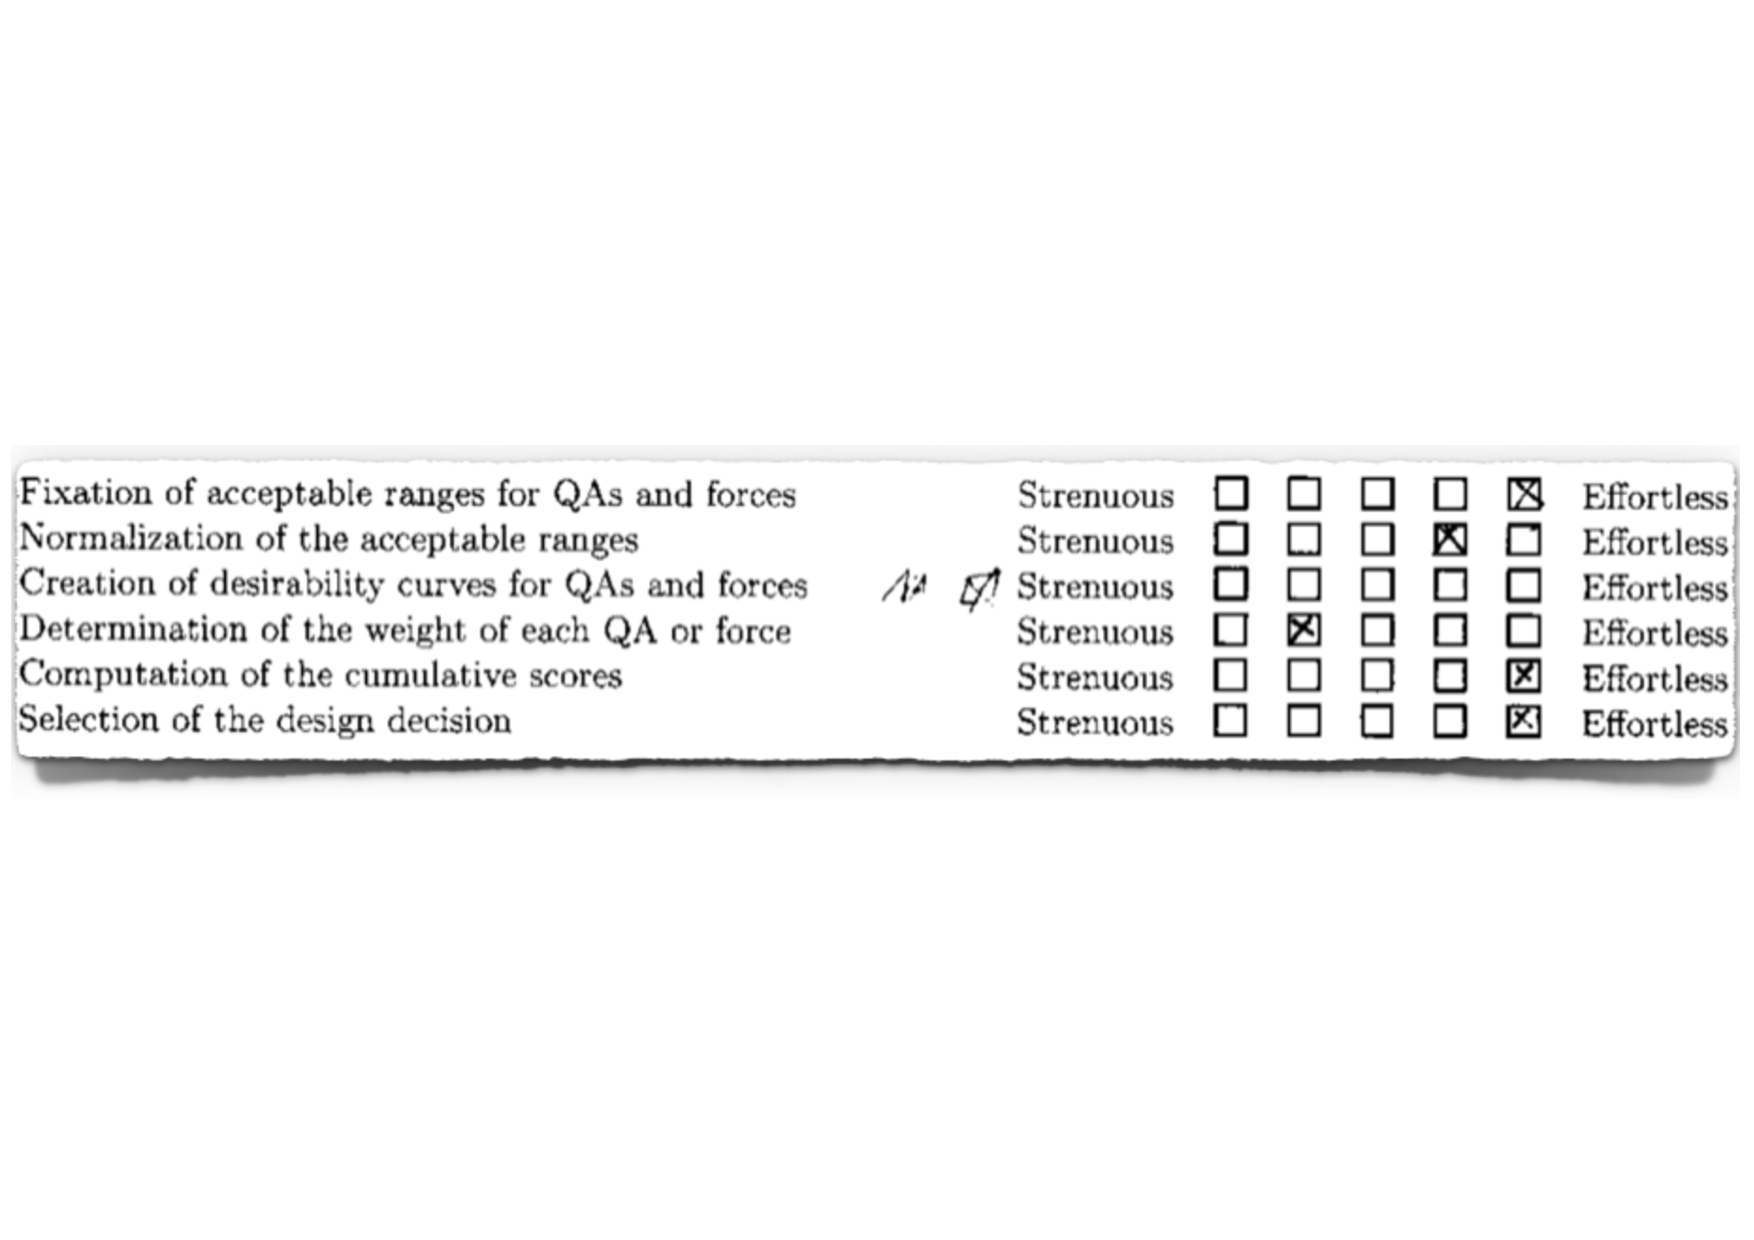
\includegraphics{questionnaire_part_1.pdf}}
  % \end{figure}  

  % \begin{tikzpicture}[font=\small]
  %   \foreach \line in {1,2} {
  %       \begin{scope}[yshift=-\line cm]
  %           \foreach \letter/\position in {\color{white}A/1, B/2, C/3, D/4, E/5} { 
  %               \node at (0,0) {\normalsize\textbf{\line}};
  %               \node[draw,rectangle,inner sep=1pt] at ({\position * 0.5},0) {\letter};
  %           }
  %       \end{scope}
  %   }
  % \end{tikzpicture}

  \begin{minipage}{10.8cm} 
  \structure{1.1 What do you think about the following steps of the decision ranking method in terms of the effort
        required to carry them out?}
  \end{minipage}

  \begin{description}
    \item Fixation of acceptable ranges for QAs/forces \tiny(Step~\structure{\ding{203}})\normalsize
    \begin{flushright}
      \begin{tikzpicture}[font=\small]
        \begin{scope}[yshift=-1 cm]
            \foreach \letter/\position in {\color{white}A/1, \color{white}B/2, \color{white}C/3, \color{white}D/4, \ding{51}/5} { 
                \node at (0,0) {\tiny Strenuous~~~~~~~~};
                \node[draw,rectangle,inner sep=1pt] at ({\position * 0.5},0) {\letter};
                \node at (3.4,0) {\tiny Effortless};
            } 
        \end{scope}
  \end{tikzpicture}
    \end{flushright}
      
    \item Normalization of the acceptable ranges \tiny(Step~\structure{\ding{204}})\normalsize 
    \begin{flushright}
      \begin{tikzpicture}[font=\small]
        \begin{scope}[yshift=-1 cm]
            \foreach \letter/\position in {\color{white}A/1, \color{white}B/2, \color{white}C/3, \ding{51}/4, \color{white}E/5} { 
                \node at (0,0) {\tiny Strenuous~~~~~~~~};
                \node[draw,rectangle,inner sep=1pt] at ({\position * 0.5},0) {\letter};
                \node at (3.4,0) {\tiny Effortless};
            } 
        \end{scope}
  \end{tikzpicture}
    \end{flushright}

    \item Creation of desirability ranges for QAs/forces \tiny(Step~\structure{\ding{205}})\normalsize
    \begin{flushright}
      \begin{tikzpicture}[font=\small]
        \begin{scope}[yshift=-1 cm]
            \foreach \letter/\position in {\color{white}A/1, \color{white}B/2, \color{white}C/3, \color{white}D/4, \color{white}E/5} { 
                \node at (0,0) {\tiny Strenuous~~~~~~~~};
                \node[draw,rectangle,inner sep=1pt] at ({\position * 0.5},0) {\letter};
                \node at (3.4,0) {\tiny Effortless};
            } 
        \end{scope}
  \end{tikzpicture}
  \end{flushright}
          
  \end{description}
  
\end{frame}

\begin{frame}\frametitle{Taking a Look at the Post-Questionnaire (2)}

  \begin{minipage}{10.8cm} 
  \structure{1.1 What do you think about the following steps of the decision ranking method in terms of the effort
        required to carry them out?}
  \end{minipage}

    \begin{description}
      
      \item Determination of the weight of each QA/force \tiny(Step~\structure{\ding{206}})\normalsize
      \begin{flushright}
        \begin{tikzpicture}[font=\small]
        \begin{scope}[yshift=-1 cm]
            \foreach \letter/\position in {\color{white}A/1, \ding{51}/2, \color{white}C/3, \color{white}D/4, \color{white}E/5} { 
                \node at (0,0) {\tiny Strenuous~~~~~~~~};
                \node[draw,rectangle,inner sep=1pt] at ({\position * 0.5},0) {\letter};
                \node at (3.4,0) {\tiny Effortless};
            } 
        \end{scope}
  \end{tikzpicture}
      \end{flushright}
          
    \item Computation of cumulative scores \tiny(Step~\structure{\ding{207}})\normalsize
    \begin{flushright}
                \begin{tikzpicture}[font=\small]
        \begin{scope}[yshift=-1 cm]
            \foreach \letter/\position in {\color{white}A/1, \color{white}B/2, \color{white}C/3, \color{white}D/4, \ding{51}/5} { 
                \node at (0,0) {\tiny Strenuous~~~~~~~~};
                \node[draw,rectangle,inner sep=1pt] at ({\position * 0.5},0) {\letter};
                \node at (3.4,0) {\tiny Effortless};
            } 
        \end{scope}
  \end{tikzpicture}
      
    \end{flushright}
    \item Selection of the design decision \tiny(Step~\structure{\ding{208}})\normalsize
    \begin{flushright}
                \begin{tikzpicture}[font=\small]
        \begin{scope}[yshift=-1 cm]
            \foreach \letter/\position in {\color{white}A/1, \color{white}B/2, \color{white}C/3, \color{white}D/4, \ding{51}/5} { 
                \node at (0,0) {\tiny Strenuous~~~~~~~~};
                \node[draw,rectangle,inner sep=1pt] at ({\position * 0.5},0) {\letter};
                \node at (3.4,0) {\tiny Effortless};
            } 
        \end{scope}
  \end{tikzpicture}      
    \end{flushright}

  \end{description}
  
\end{frame}

\begin{frame}\frametitle{Taking a Look at the Post-Questionnaire (3)}

  \begin{minipage}{10.8cm} 
  \structure{1.2 How do you rate the overall effort required to carry out the decision ranking method?}
  \end{minipage}
  \begin{description}
    \item \color{white}AAAA\color{black}
    \begin{flushright}
                \begin{tikzpicture}[font=\small]
        \begin{scope}[yshift=-1 cm]
            \foreach \letter/\position in {\color{white}A/1, \color{white}B/2, \ding{51}/3, \color{white}D/4, \color{white}D/5} { 
                \node at (0,0) {\tiny Strenuous~~~~~~~~};
                \node[draw,rectangle,inner sep=1pt] at ({\position * 0.5},0) {\letter};
                \node at (3.4,0) {\tiny Effortless};
            } 
        \end{scope}
  \end{tikzpicture}      
    \end{flushright}
  \end{description}

  \vspace{0.3cm}
  \begin{minipage}{10.8cm} 
  \structure{1.3 The results made it easy for me to better evaluate the trade-offs among the decisions and their architectural implications?}
  \end{minipage}
  \begin{description}
    \item \color{white}AAAA\color{black}
    \begin{flushright}
                \begin{tikzpicture}[font=\small]
        \begin{scope}[yshift=-1 cm]
            \foreach \letter/\position in {\color{white}A/1, \color{white}B/2, \ding{51}/3, \color{white}D/4, \color{white}D/5} { 
                \node at (0,0) {\tiny Strongly agree~~~~~~~~~~~~};
                \node[draw,rectangle,inner sep=1pt] at ({\position * 0.5},0) {\letter};
                \node at (3.4,0) {\tiny ~~~~~Strongly disagree};
            } 
        \end{scope}
  \end{tikzpicture}      
    \end{flushright}
  \end{description}

\end{frame}

\begin{frame}\frametitle{Taking a Look at the Post-Questionnaire (4)}
  \framesubtitle{Free-form Questions}
  \begin{minipage}{10.8cm} 
  \structure{2.1 What are the major strengths of the decisions ranking method?}
  \end{minipage}

  \textbf{R.} \ding{125}Structured way to identify relative priorities of forces.\ding{126}

  \vspace{.3cm}
  \begin{minipage}{10.8cm} 
  \structure{2.2 What are the major drawbacks of the decision ranking method?}
  \end{minipage}
  \begin{minipage}{10.80cm}
    \textbf{R.} \ding{125}[...] coming up with \emph{HE decisions} is not as trivial and 
    already requires that the weight of the forces is known [...]\ding{126}
    \vspace{0.2cm}
    \par \ding{125}
    I am wondering if stakeholders could come up with HE decisions 
    why do they need to rank forces in the first place?\ding{126} 
    \vspace{0.2cm}
    \par \ding{125}
    [...] this method requires more effort if more than three forces 
    need to be considered. It seems that it does not scale that well.\ding{126}

  \end{minipage}
\end{frame}


\begin{frame}\frametitle{Taking a Look at the Post-Questionnaire (5)}
  \framesubtitle{Free-form Questions}
  \begin{minipage}{10.8cm} 
  \structure{2.3 Do you have any comments regarding the practical difficulties of 
  applying the decision ranking method?}
  \end{minipage}

  \begin{minipage}{10.8cm}
    \vspace{.15cm}
    \textbf{R.} \ding{125}[...] it seems as if this method produces the best result if it is performed by a group of people 
  (of the same stakeholder group)\newline 
  \par [...] but we couldn't try this scenario in the pilot.\ding{126}
  \end{minipage}

\end{frame}

\section{A ferramenta KDM-RE} 
\label{sec:where_to_go_from_here_}
\frame{\tableofcontents[currentsection]}


% \definecolor{myblue}{RGB}{83,121,200}

\tikzset{
myshape/.style={
  shape=signal,
  fill=blue!63,
  minimum height=1.5cm,
  minimum width=1.5cm,
  text=white,
  signal pointer angle=130,
  signal to=east,
  signal from=west,
  rotate=-90,
  transform shape
  },
mytext/.style={
  draw=blue!63,
  text width=7cm,
  minimum height=1.15cm,
  thick,
  outer sep=0pt
  }  
}
\newcounter{tmp}
\newcommand\MyDesc[3][]{
\stepcounter{tmp}%
\node[myshape,#1] (desc\thetmp) {};
\node[font=\color{white}] at (desc\thetmp) {#2};
\node[mytext,anchor=north west] at (desc\thetmp.north west) 
  {%
    \parbox[t]{2em}{\hfill$\bullet$\hfill\null}%
    \parbox[t]{\dimexpr\linewidth-2em\relax}{#3}%
  };
}

\begin{frame}[plain]\frametitle{Interpreting the Results: The HE Seems to be the Problem\ldots}
  
\setbeamercolor{footnote mark}{fg=white}

Characterization schema: commonalities and variabilities
\vspace{.2cm}

\begin{tikzpicture}[]

  \MyDesc{\tiny Description}{Step: \structure{\ding{202}}}

  \MyDesc[below = 1.5cm of desc1.north]{\tiny Importance}{Steps: \structure{\ding{203}}, \structure{\ding{204}}}

  \MyDesc[below = 1.5cm of desc2.north]{\tiny Fitness{\footnote{$^1$ Fulfillment.}}}{Steps: \structure{\ding{205}}, \structure{\ding{206}}}

  \uncover<2-3>{
  \MyDesc[below = 1.5cm of desc2.north]{\tiny Fitness$^1$}{Steps: \structure{\ding{205}}, \textbf{\color{red}X}}
  }

  \uncover<3>{
  \MyDesc[below = 1.5cm of desc3.north]{\tiny Uncertainty}{Steps: 
  so far, none.}
  }
\end{tikzpicture}
\end{frame}

% \begin{frame}\frametitle{}

% \begin{minipage}{10.8cm}
% At this point, we want something that \textbf{avoids the selection of a worse alternative} and, at the same time, it is \textbf{easy to use}. 
% \end{minipage}

% \begin{itemize}
%   \item todo
%   \item todo
%   \item todo
%   \item todo  
% \end{itemize}
% \end{frame}

\section{Avaliação}
\label{sec:wrapping_up}

\begin{frame}\frametitle{Concluding Remarks\ldots}
  \begin{itemize}
    \begin{minipage}{9.8cm}\item Provides a systematic way to ponder about decisions;\vspace{0.2cm}\end{minipage}
    \begin{minipage}{9.8cm}\item \textbf{Quantitative overview} of how each decision performs on 
    important QAs/forces;\vspace{0.2cm}\end{minipage}
    \begin{minipage}{9.8cm}\item \textbf{Downside:} highly \textbf{``mathy''}, \textbf{cumbersome};\vspace{0.2cm}\end{minipage}
    \begin{minipage}{9.8cm}\item \textbf{Future:} 
    Replace the HE method and carry out an \textbf{empirical study} to evaluate how well the ranking method works for graduate students.\vspace{0.2cm}\end{minipage} 
  \end{itemize}
\end{frame}

\section{Conclusões}
\subsection{Contribuições, Limitações, Trabalhos Futuros e Publicações}


\begin{frame}[plain,c]\frametitle{}
\begin{center}
% Well that brings me to the end of the presentation. 
% Thank you for your attention.
\Huge
``What a Long, Strange Trip It's Been''\footnote{
  \textbf{\tiny What a Long, Strange Trip It's Been}, by Grateful Dead, is arguably one of the most famous lines in rock and roll. This snippet has entitled several books and articles since the song's release. Since it evokes a lifespan of constant changes, I believe it fits perfectly to describe my stay here.
  } \\
  \pause
\Huge \textbf{Thank you!}
\smiley
\end{center}
  
\end{frame}

\begin{frame}\frametitle{Bibliografia}
  % estilo da bibliografia
  \bibliographystyle{abbrv}
  % chamando o arquivo refs.bib
  \bibliography{references}
\end{frame}

% \frame[plain,c]{
% \begin{center}
% % Well that brings me to the end of the presentation. 
% % Thank you for your attention.
% \Huge \textbf{Thank you!}
% \smiley
% \end{center}
% }

\end{document}
